\documentclass[color=usenames,dvipsnames]{beamer}\usepackage[]{graphicx}\usepackage[]{color}
% maxwidth is the original width if it is less than linewidth
% otherwise use linewidth (to make sure the graphics do not exceed the margin)
\makeatletter
\def\maxwidth{ %
  \ifdim\Gin@nat@width>\linewidth
    \linewidth
  \else
    \Gin@nat@width
  \fi
}
\makeatother

\definecolor{fgcolor}{rgb}{0.345, 0.345, 0.345}
\newcommand{\hlnum}[1]{\textcolor[rgb]{0.686,0.059,0.569}{#1}}%
\newcommand{\hlstr}[1]{\textcolor[rgb]{0.192,0.494,0.8}{#1}}%
\newcommand{\hlcom}[1]{\textcolor[rgb]{0.678,0.584,0.686}{\textit{#1}}}%
\newcommand{\hlopt}[1]{\textcolor[rgb]{0,0,0}{#1}}%
\newcommand{\hlstd}[1]{\textcolor[rgb]{0.345,0.345,0.345}{#1}}%
\newcommand{\hlkwa}[1]{\textcolor[rgb]{0.161,0.373,0.58}{\textbf{#1}}}%
\newcommand{\hlkwb}[1]{\textcolor[rgb]{0.69,0.353,0.396}{#1}}%
\newcommand{\hlkwc}[1]{\textcolor[rgb]{0.333,0.667,0.333}{#1}}%
\newcommand{\hlkwd}[1]{\textcolor[rgb]{0.737,0.353,0.396}{\textbf{#1}}}%
\let\hlipl\hlkwb

\usepackage{framed}
\makeatletter
\newenvironment{kframe}{%
 \def\at@end@of@kframe{}%
 \ifinner\ifhmode%
  \def\at@end@of@kframe{\end{minipage}}%
  \begin{minipage}{\columnwidth}%
 \fi\fi%
 \def\FrameCommand##1{\hskip\@totalleftmargin \hskip-\fboxsep
 \colorbox{shadecolor}{##1}\hskip-\fboxsep
     % There is no \\@totalrightmargin, so:
     \hskip-\linewidth \hskip-\@totalleftmargin \hskip\columnwidth}%
 \MakeFramed {\advance\hsize-\width
   \@totalleftmargin\z@ \linewidth\hsize
   \@setminipage}}%
 {\par\unskip\endMakeFramed%
 \at@end@of@kframe}
\makeatother

\definecolor{shadecolor}{rgb}{.97, .97, .97}
\definecolor{messagecolor}{rgb}{0, 0, 0}
\definecolor{warningcolor}{rgb}{1, 0, 1}
\definecolor{errorcolor}{rgb}{1, 0, 0}
\newenvironment{knitrout}{}{} % an empty environment to be redefined in TeX

\usepackage{alltt}
%\documentclass[color=usenames,dvipsnames,handout]{beamer}

%\usepackage[roman]{../pres1}
\usepackage[sans]{../pres1}


\usepackage{changepage}


%\newcommand{\wide}{\column{\dimexpr\paperwidth}} % Must be in columns environment




\IfFileExists{upquote.sty}{\usepackage{upquote}}{}
\begin{document}


\setlength\fboxsep{0pt}


{
\usebackgroundtemplate{
  \parbox[c][\paperheight][b]{\paperwidth}{
    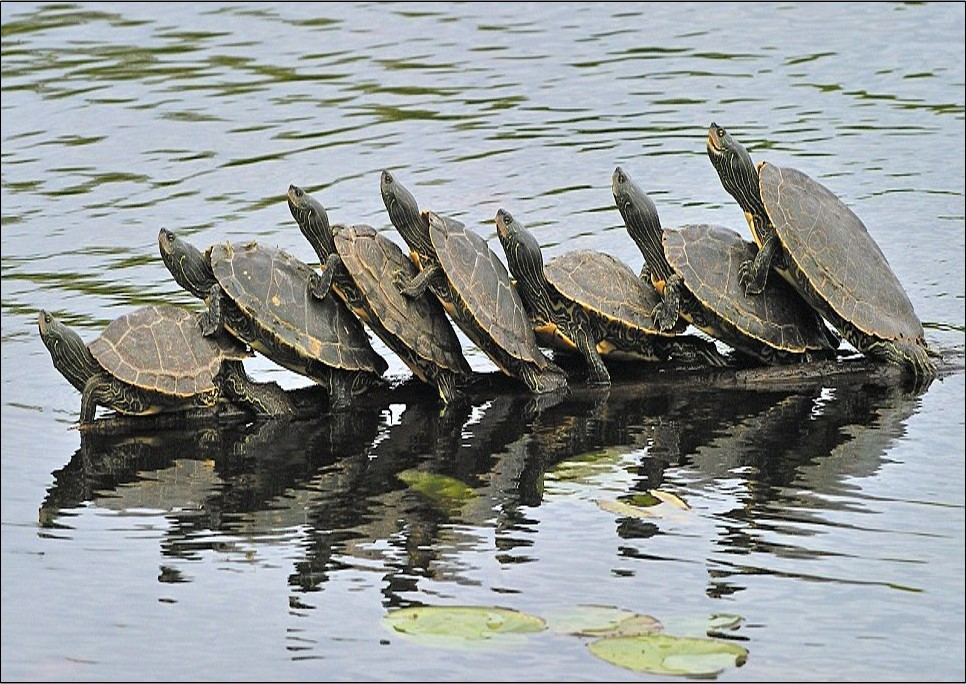
\includegraphics[width=\paperwidth,trim=0mm 0mm 0mm 0cm,clip]{figs/turtles}}
  }
\begin{frame}[plain]
  \vspace{-2.35cm}
  \begin{center}
    {\huge Logistic Population Growth } \\
  \end{center}
  \begin{adjustwidth}{-1cm}{-1cm}
    \rule[-7mm]{\paperwidth}{0.5pt}
  \end{adjustwidth}
\end{frame}
}





\section{Background}



\begin{frame}[plain]
  \frametitle{Learning objectives}
  \Large
  The equation for logistic growth in discrete time \\
  \pause
  \vfill
  The definition of density-dependent growth \\
  \pause
  \vfill
  Basic properties of the model \\
  \pause
  \vfill
  Strange behavior of the (discrete time) model, such as damped oscillations and chaos \\
\end{frame}



\section{Logistic growth}


\begin{frame}
  \frametitle{From Geometric to Logistic Growth}
  \large
  {\bf Geometric growth}
  \[
    N_{t+1} = N_t + N_tr
  \]
  \pause
  {\bf Logistic growth}
  \[
    N_{t+1} = N_t + N_t r_{max}\left(1 - \frac{N_t}{K}\right)
  \]
  where \\
  \begin{itemize}
    \item $r_{max}$ is the growth rate when $N_t$ is close to 0. \\
    \item $K$ is the carrying capacity
  \end{itemize}
\end{frame}





\begin{frame}
  \frametitle{Density-dependent growth}
  \large
  Logistic growth is an example of {\bf density-dependent
    growth} \\
  \vspace{0.5cm}
  \visible<2->{\textbf{Definition:} Population growth rate %($\lambda$)
    {\it is}  affected by population size ($N$).} \\
  \vspace{0.5cm}
  \visible<3->{\textbf{Implications}:  Resources are limited and there
    is a carrying capacity.} \\
\end{frame}




\begin{frame}[fragile]
  \frametitle{Graphical depiction}




\vspace{-1cm}
\begin{center}
  \only<1 | handout:0>{\includegraphics[width=0.8\textwidth]{figure/geom-1}}
  \only<2>{\includegraphics[width=0.8\textwidth]{figure/geom-logistic-1}}
\end{center}
\end{frame}








\begin{frame}[fragile]
  \frametitle{Growth rate ($\lambda_t = N_{t+1}/N_t$)}


\begin{center}
  \includegraphics[width=\textwidth]{figure/lr1-1} \\ \vfill
  \includegraphics[width=\textwidth]{figure/lambda-1}
\end{center}
\end{frame}







\begin{frame}[fragile]
  \frametitle{Growth ($\Delta_t=N_{t+1}-N_t$)}


\begin{center}
  \includegraphics[width=\textwidth]{figure/lr2-1} \\ \vfill
  \includegraphics[width=\textwidth]{figure/delta-1}
\end{center}
\end{frame}



\begin{frame}[fragile]
  \frametitle{Growth ($\Delta_t=N_{t+1}-N_t$) as a function of $N$}

\begin{center}
  \includegraphics[width=\textwidth]{figure/delta-N-1}
\end{center}
\end{frame}






\begin{frame}[fragile]
  \frametitle{What happens when we change $r_{max}$?}





\begin{center}
  \only<1|handout:0>{\includegraphics[width=\textwidth]{figure/Nl-1}}
  \only<2|handout:0>{\includegraphics[width=\textwidth]{figure/Nl2-1}}
  \only<3|handout:0>{\includegraphics[width=\textwidth]{figure/Nl3-1}}
  \only<4>{\includegraphics[width=\textwidth]{figure/Nl4-1}}
\end{center}
\end{frame}





\begin{frame}
  \frametitle{Definitions}
  \begin{block}{Overcompensation}
    Density-dependent response in which populations over- or
    under-shoot carrying capacity rather than approach it gradually
  \end{block}
  \pause
  \begin{block}{Chaos}
    Highly variable deterministic dynamics that are extremely
    sensitive to small changes in parameters
  \end{block}
\end{frame}






%\begin{frame}
%  \frametitle{Allee effects}%
%
%\end{frame}





%\section{Assumptions}

\begin{frame}
  \frametitle{Assumptions of basic model}
  \Large
  \begin{itemize}
    \item $K$ and $r_{max}$ are constant
    \item No sex or age effects or other sources of individual heterogeneity
    \item No time lags
    \item No stochasticity
%    \item Crowding affects all members of the population equally
  \end{itemize}
\end{frame}




%% This section is ignored for now
\begin{comment}

\section{Population Cycles}






\begin{frame}
  \frametitle{Population cycles}
  \centering
  \fbox{\includegraphics[width=0.7\textwidth]{figs/Lemmus_Lemmus}} \par
\end{frame}



\begin{frame}
  \frametitle{Population cycles}
  {\centering \bf Voles and Lemmings \par}
  \includegraphics[width=\textwidth]{figs/vole_lemming_cycles_Stenseth99} \par
\end{frame}



\begin{frame}
  \frametitle{Population cycles}
  {\centering \bf Insects, voles, and grouse \par}
  \includegraphics[width=\textwidth]{figs/cyclic_populations} \par
\end{frame}



\begin{frame}
  \frametitle{Real-world population cycles}
  {\centering \bf Soay sheep \par}
  \begin{center}
    \includegraphics[width=0.6\textwidth]{../cyclesI/figs/Soay_sheep_Grenfell92}
    \fbox{\includegraphics[width=0.4\textwidth]{figs/Soay_sheep_lamb}}
  \end{center}
\end{frame}






%\subsection{Time lags}

\begin{frame}
  \frametitle{Population cycles -- Time lags}
  {\bf Logistic growth with time lag}
  \[
    N_{t+1} = N_t + N_t r_{max}\left(1 - \frac{N_{t-lag}}{K}\right)
  \]
  where \\
  \begin{itemize}
    \item $r_{max}$ is the growth rate when $N_t$ is close to 0. \\
    \item $K$ is the carrying capacity
    \item $lag$ is an integer (0,1,2,\dots) used to reference earlier
      time point
  \end{itemize}
\end{frame}



\begin{frame}[fragile]
  \frametitle{Time lags}

\begin{center}
  \includegraphics[width=\textwidth]{figure/Nl5-1}
\end{center}
\end{frame}


%\subsection{Cyclic carrying capacity}


\begin{frame}
  \frametitle{Population cycles -- cyclic carrying capacity}
  {\bf Carrying capacity changes every year}
  \begin{gather*}
    K_t = k_0 + k_1\cos\left(\frac{2 \pi t}{c}\right) \\
    \uncover<2>{N_{t+1} = N_t + N_t r_{max}\left(1 - \frac{N_t}{K_t}\right)}
  \end{gather*}
\end{frame}





%% \begin{frame}[fragile]
%%   \frametitle{Cyclic carrying capacity}
%% <<Nl6,include=FALSE,echo=FALSE,width=8,height=6>>=
%% Nl6 <- Nl
%% Nl6[1] <- 50
%% k0 <- K
%% k1 <- 10
%% c <- 20
%% Kt <- numeric(T)
%% for(t in 2:T) {
%%     Kt[t] <- k0 + k1*cos(2*pi*t/c)
%%     Nl6[t] <- Nl6[t-1] + Nl6[t-1]*1.1*(1-Nl6[t-1]/Kt[t])
%% }
%% plot(Nl6, type="o", xlab="Time (t)", ylab="Population size (N)",
%%      cex.lab=1.3, panel.first=abline(h=K, col="blue", lty=2),
%%      col="steelblue", lwd=4, main="r=1.1, k0=50, k1=10, c=20")
%% @
%% \begin{center}
%%   \includegraphics[width=\textwidth]{logistic-growth-Nl6}
%% \end{center}
%% \end{frame}








\begin{frame}[fragile]
  \frametitle{Cyclic carrying capacity}


\begin{center}
  \only<1>{\includegraphics[width=\textwidth]{figure/Nl6-1}}
  \only<2>{\includegraphics[width=\textwidth]{figure/Nl6-2-1}}
\end{center}
\end{frame}






\end{comment}








\section{Summary}


%% \begin{frame}
%%   \frametitle{Regulated or limited?}
%%   \begin{block}{Regulated}

%%   \end{block}
%%   \begin{block}{Limited}

%%   \end{block}
%% \end{frame}



\begin{frame}
  \frametitle{Summary and assignment}
  \large
  {\bf Summary}
  \begin{itemize}[<+->]
    \item Logistic growth is a form of density-dependent growth
    \item Growth rate ($\lambda_t=N_{t+1}/N_t$) declines as $N$ approaches $K$
    \item Growth ($\Delta_t=N_{t+1}-N_t$) peaks at $K/2$ (the
      inflection point)
    \item The model isn't mechanistic in the sense that it doesn't
      include birth, mortality, and movement processes. 
    \item But it does allow for complex dynamics that resemble
      patterns seen in nature.
  \end{itemize}
  \vfill
  \uncover<6->{
  {\bf Assignment \par}
  Read pages 32--36 in Conroy and Carroll \par
  }
\end{frame}




\end{document}
